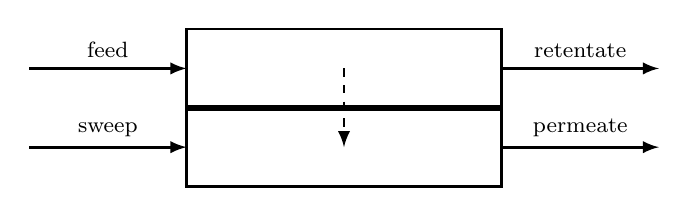
\begin{tikzpicture}[arrow/.style={line width=1pt,->,>=latex}]
	\draw [line width=1pt] (-2,2) rectangle (2,0);
	\draw [arrow] (-4,1.5) -- (-2,1.5) node [pos=0.5, above] {\footnotesize feed};
	\draw [arrow] (-4,0.5) -- (-2,0.5) node [pos=0.5, above] {\footnotesize sweep};
	\draw [arrow] (2,1.5) -- (4,1.5) node [pos=0.5, above] {\footnotesize retentate};
	\draw [arrow] (2,0.5) -- (4,0.5) node [pos=0.5, above] {\footnotesize permeate};
	\draw [line width=2pt] (-2,1) -- (2,1);
	\draw [line width=1pt,->,>=latex,dashed] (0,1.5)  -- (0,0.5) node [pos=0.5, left] {\footnotesize }; 
\end{tikzpicture}�